% This file was created with tikzplotlib v0.10.1.
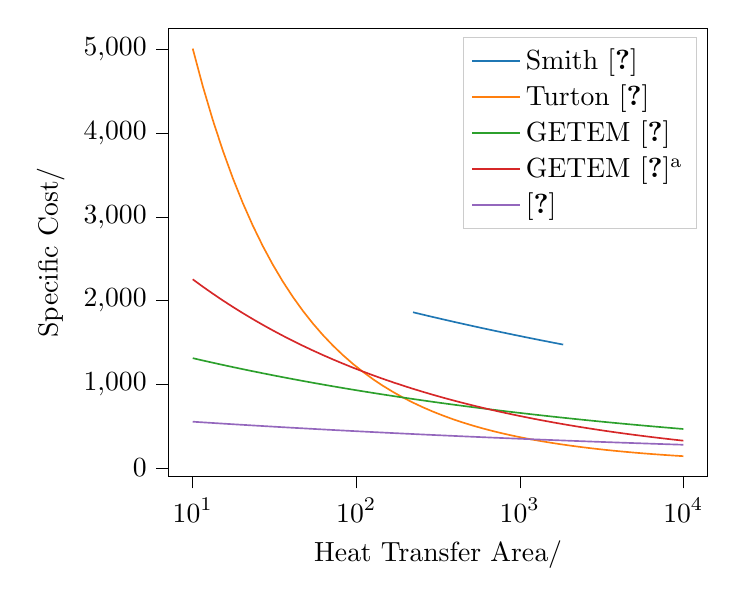
\begin{tikzpicture}

\definecolor{crimson2143940}{RGB}{214,39,40}
\definecolor{darkgray176}{RGB}{176,176,176}
\definecolor{darkorange25512714}{RGB}{255,127,14}
\definecolor{forestgreen4416044}{RGB}{44,160,44}
\definecolor{lightgray204}{RGB}{204,204,204}
\definecolor{mediumpurple148103189}{RGB}{148,103,189}
\definecolor{steelblue31119180}{RGB}{31,119,180}

\begin{axis}[
legend cell align={left},
legend style={fill opacity=0.8, draw opacity=1, text opacity=1, draw=lightgray204},
log basis x={10},
tick align=outside,
tick pos=left,
unbounded coords=jump,
x grid style={darkgray176},
xlabel={Heat Transfer Area/\unit{\square\m}},
xmin=7.07945784384138, xmax=14125.3754462276,
xmode=log,
xtick style={color=black},
xtick={0.1,1,10,100,1000,10000,100000,1000000},
xticklabels={
  \(\displaystyle {10^{-1}}\),
  \(\displaystyle {10^{0}}\),
  \(\displaystyle {10^{1}}\),
  \(\displaystyle {10^{2}}\),
  \(\displaystyle {10^{3}}\),
  \(\displaystyle {10^{4}}\),
  \(\displaystyle {10^{5}}\),
  \(\displaystyle {10^{6}}\)
},
y grid style={darkgray176},
ylabel={Specific Cost/\unit{\USD\per\square\m}},
ymin=-102.998946756242, ymax=5254.02836911878,
ytick style={color=black}
]
\addplot [semithick, steelblue31119180]
table {%
10 nan
11.5139539932645 nan
13.2571136559011 nan
15.2641796717523 nan
17.5751062485479 nan
20.2358964772516 nan
23.2995181051537 nan
26.8269579527973 nan
30.8884359647748 nan
35.5648030622313 nan
40.9491506238043 nan
47.1486636345739 nan
54.2867543932386 nan
62.5055192527397 nan
71.9685673001152 nan
82.8642772854684 nan
95.4095476349994 nan
109.854114198756 nan
126.48552168553 nan
145.634847750124 nan
167.683293681101 nan
193.069772888325 nan
222.29964825262 1860.06471639853
255.954792269954 1831.44280665977
294.705170255181 1803.26131907937
339.322177189533 1775.51347662256
390.693993705462 1748.19260653678
449.843266896944 1721.29213874706
517.947467923121 1694.80560427602
596.362331659464 1668.72663368823
686.6488450043 1643.04895555853
790.60432109077 1617.76639496385
910.298177991522 1592.8728719983
1048.11313415469 1568.36240031109
1206.79264063933 1544.22908566692
1389.49549437314 1520.46712452854
1599.85871960606 1497.07080266116
1842.06996932672 1474.03449375827
2120.95088792019 nan
2442.05309454865 nan
2811.76869797423 nan
3237.45754281764 nan
3727.59372031494 nan
4291.93426012878 nan
4941.71336132383 nan
5689.86602901829 nan
6551.28556859551 nan
7543.12006335462 nan
8685.11373751352 nan
10000 nan
};
\addlegendentry{Smith \cite{Smith2005}}
\addplot [semithick, darkorange25512714]
table {%
10 5010.5271274881
11.5139539932645 4563.13789134132
13.2571136559011 4159.26280555285
15.2641796717523 3794.38790095293
17.5751062485479 3464.49298268143
20.2358964772516 3165.99511147049
23.2995181051537 2895.69881654733
26.8269579527973 2650.75220945449
30.8884359647748 2428.60827393442
35.5648030622313 2226.99069898662
40.9491506238043 2043.86370215134
47.1486636345739 1877.40535961592
54.2867543932386 1725.98402027147
62.5055192527397 1588.13743356655
71.9685673001152 1462.55426694931
82.8642772854684 1348.05772875437
95.4095476349994 1243.59104734953
109.854114198756 1148.20458787988
126.48552168553 1061.04441461194
145.634847750124 981.342130190062
167.683293681101 908.405843505824
193.069772888325 841.612135725501
222.29964825262 780.398909647704
255.954792269954 724.259021257029
294.705170255181 672.734604345742
339.322177189533 625.412009609213
390.693993705462 581.917288867463
449.843266896944 541.912163187184
517.947467923121 505.090420816982
596.362331659464 471.174697125964
686.6488450043 439.913594259562
790.60432109077 411.079103089667
910.298177991522 384.464294320509
1048.11313415469 359.881249388232
1206.79264063933 337.159205122827
1389.49549437314 316.142889080587
1599.85871960606 296.691025050686
1842.06996932672 278.674990532694
2120.95088792019 261.977610008998
2442.05309454865 246.492069629273
2811.76869797423 232.120940511057
3237.45754281764 218.775299265843
3727.59372031494 206.373935605216
4291.93426012878 194.842637985522
4941.71336132383 184.113549228648
5689.86602901829 174.124584925641
6551.28556859551 164.818908201614
7543.12006335462 156.14445510612
8685.11373751352 148.053505502803
10000 140.502294874441
};
\addlegendentry{Turton \cite{Turton2012}}
\addplot [semithick, forestgreen4416044]
table {%
10 1311.73056360972
11.5139539932645 1284.28368161225
13.2571136559011 1257.41110302149
15.2641796717523 1231.10081101154
17.5751062485479 1205.34104019867
20.2358964772516 1180.1202713801
23.2995181051537 1155.42722638292
26.8269579527973 1131.25086302066
30.8884359647748 1107.58037015555
35.5648030622313 1084.40516286395
40.9491506238043 1061.71487770305
47.1486636345739 1039.49936807652
54.2867543932386 1017.74869969724
62.5055192527397 996.453146144835
71.9685673001152 975.603184516291
82.8642772854684 955.189491167489
95.4095476349994 935.202937543888
109.854114198756 915.634586098432
126.48552168553 896.475686294884
145.634847750124 877.717670694766
167.683293681101 859.352151126202
193.069772888325 841.370914932901
222.29964825262 823.765921301646
255.954792269954 806.529297666615
294.705170255181 789.653336188943
339.322177189533 773.130490309948
390.693993705462 756.953371376473
449.843266896944 741.114745336848
517.947467923121 725.607529505974
596.362331659464 710.424789398108
686.6488450043 695.559735625913
790.60432109077 681.005720864387
910.298177991522 666.756236878336
1048.11313415469 652.804911612025
1206.79264063933 639.14550633974
1389.49549437314 625.771912875966
1599.85871960606 612.67815084394
1842.06996932672 599.858365001358
2120.95088792019 587.306822622043
2442.05309454865 575.017910932389
2811.76869797423 562.986134601459
3237.45754281764 551.206113283591
3727.59372031494 539.672579212426
4291.93426012878 528.380374845277
4941.71336132383 517.324450556792
5689.86602901829 506.499862380873
6551.28556859551 495.901769799841
7543.12006335462 485.525433579863
8685.11373751352 475.366213651673
10000 465.419567035633
};
\addlegendentry{GETEM \cite{GETEM2016}}
\addplot [semithick, crimson2143940]
table {%
10 2253.73796240069
11.5139539932645 2166.50932652656
13.2571136559011 2082.65678629593
15.2641796717523 2002.04967336027
17.5751062485479 1924.56237675661
20.2358964772516 1850.07414716653
23.2995181051537 1778.46890875122
26.8269579527973 1709.63507826913
30.8884359647748 1643.46539119463
35.5648030622313 1579.85673456644
40.9491506238043 1518.7099863056
47.1486636345739 1459.92986075243
54.2867543932386 1403.42476018177
62.5055192527397 1349.1066320653
71.9685673001152 1296.89083185823
82.8642772854684 1246.69599109681
95.4095476349994 1198.44389060093
109.854114198756 1152.05933858431
126.48552168553 1107.47005348227
145.634847750124 1064.6065513146
167.683293681101 1023.40203740788
193.069772888325 983.792302308595
222.29964825262 945.715621724821
255.954792269954 909.112660340595
294.705170255181 873.92637935301
339.322177189533 840.101947588022
390.693993705462 807.586656056414
449.843266896944 776.329835816798
517.947467923121 746.282779017631
596.362331659464 717.398662995232
686.6488450043 689.632477309499
790.60432109077 662.940953603641
910.298177991522 637.282498178616
1048.11313415469 612.617127177203
1206.79264063933 588.906404276711
1389.49549437314 566.113380793235
1599.85871960606 544.202538104102
1842.06996932672 523.139732298808
2120.95088792019 502.892140972185
2442.05309454865 483.428212076875
2811.76869797423 464.717614755427
3237.45754281764 446.731192075384
3727.59372031494 429.440915593705
4291.93426012878 412.819841679736
4941.71336132383 396.842069528646
5689.86602901829 381.482700799914
6551.28556859551 366.71780081797
7543.12006335462 352.524361274518
8685.11373751352 338.880264374441
10000 325.764248369385
};
\addlegendentry{GETEM \cite{GETEM2016}\textsuperscript{a}}
\addplot [semithick, mediumpurple148103189]
table {%
10 552.545665381231
11.5139539932645 544.810824009667
13.2571136559011 537.184259247244
15.2641796717523 529.6644553778
17.5751062485479 522.249917903008
20.2358964772516 514.939173245361
23.2995181051537 507.730768455308
26.8269579527973 500.623270922494
30.8884359647748 493.615268091041
35.5648030622313 486.705367178811
40.9491506238043 479.892194900608
47.1486636345739 473.174397195242
54.2867543932386 466.550638956427
62.5055192527397 460.019603767435
71.9685673001152 453.579993639473
82.8642772854684 447.230528753714
95.4095476349994 440.969947206949
109.854114198756 434.797004760791
126.48552168553 428.710474594392
145.634847750124 422.709147060626
167.683293681101 416.791829445679
193.069772888325 410.957345732008
222.29964825262 405.204536364618
255.954792269954 399.532258020608
294.705170255181 393.939383381948
339.322177189533 388.424800911432
390.693993705462 382.987414631769
449.843266896944 377.626143907768
517.947467923121 372.33992323157
596.362331659464 367.127702010887
686.6488450043 361.988444360206
790.60432109077 356.921128894916
910.298177991522 351.924748528314
1048.11313415469 346.998310271458
1206.79264063933 342.140835035817
1389.49549437314 337.351357438683
1599.85871960606 332.628925611317
1842.06996932672 327.972601009761
2120.95088792019 323.381458228324
2442.05309454865 318.854584815652
2811.76869797423 314.391081093398
3237.45754281764 309.990059977407
3727.59372031494 305.650646801425
4291.93426012878 301.371979143262
4941.71336132383 297.153206653392
5689.86602901829 292.993490885955
6551.28556859551 288.892005132121
7543.12006335462 284.847934255792
8685.11373751352 280.860474531597
10000 276.928833485159
};
\addlegendentry{\cite{Astolfi2014B}}
\end{axis}

\end{tikzpicture}
